\documentclass[11pt,a4paper]{article}

\usepackage[a4paper,margin=2.2cm]{geometry}
\usepackage{booktabs}
\usepackage{graphicx}
\usepackage{subcaption}
\usepackage{amsmath,amssymb}
\usepackage{siunitx}
\usepackage[hidelinks]{hyperref}
\usepackage{xcolor}
\usepackage{caption}
\usepackage{float}
\usepackage{microtype}
\usepackage{setspace}
\setstretch{1.02}

\definecolor{mpcblue}{HTML}{1D4ED8}
\newcommand{\mpcbest}[1]{\textcolor{mpcblue}{\textbf{#1}}}
\newcommand{\unitC}{\si{\celsius}}

\captionsetup{font=small,labelfont=bf}
\captionsetup[sub]{font=scriptsize,labelfont=bf}
\setlength{\floatsep}{8pt plus 2pt minus 2pt}
\setlength{\textfloatsep}{10pt plus 2pt minus 2pt}
\setlength{\intextsep}{8pt plus 2pt minus 2pt}
\setlength{\abovecaptionskip}{4pt}
\setlength{\belowcaptionskip}{2pt}

\title{%
  Offset-Free Model Predictive Control for an Induction Heater:\\
  Comparison with Hand-Tuned and Optimised PID}
\author{%
  Vinayak Raizada\\
  Department of Electrical Engineering, IIT Roorkee\\
  Industrial Control (course project)\\[0.4em]
  {\small Author roll number: \texttt{[ROLL NUMBER]} \quad Date: 31 October 2026}}
\date{}

\begin{document}
\maketitle
\thispagestyle{empty}

\begin{abstract}
Model predictive control (MPC) plans the next actuator move by rolling a plant model forward over a finite horizon and solving a constrained optimisation at every sample.
This report builds an offset-free SISO MPC for a lumped induction heater, simulates it against a nonlinear CasADi heat-balance twin, and compares it with a hand-tuned discrete PID and a SciPy-optimised PID that minimises integrated absolute error (IAE) plus a violation penalty on the same plant, seed, and limits.
After a documented retune (reference preview over the horizon, prediction length \(N{=}40\), terminal weight \(Q_t{=}50\)), MPC records the lowest IAE on setpoint tracking (\(1044\) vs \(1466\) optimised PID vs \(2477\) hand-tuned PID), on the power-limit case (\(8727\) vs \(9033\) vs \(9153\)), and under model mismatch (\(1214\) vs \(1667\) vs \(2541\)), with zero constraint violations wherever limits bind.
Optimised PID still edges MPC on two disturbance IAE numbers when it is retuned on those exact scenarios; those rows are reported without emphasis.
The verdict for this constrained heater is that MPC is the better controller: it keeps the coil inside the power window and slew limit by construction, recovers faster after mismatch, and no longer trails a scenario-tuned PID on the main tracking metrics once the horizon is allowed to see the future setpoint.
\end{abstract}

\section{Introduction}
Induction heaters are slow thermal plants with hard coil-power and slew limits.
A PID loop only reacts after temperature has already drifted, and clipping the actuator after the fact does not undo an infeasible command.
MPC uses a model to anticipate the temperature trajectory under candidate power profiles, re-optimises every sample (receding horizon), and can treat window and rate limits as hard constraints inside the optimiser~\cite{rawlings2017,camacho2013}.

The project implements that idea for coursework: an identified discrete linear model with an integrating disturbance estimate~\cite{pannocchia2003}, a SciPy quadratic programme, a CasADi heater twin as the truth plant, batch metrics, a three-screen Streamlit lab, and an animation driven by the same simulation JSON.
All physical numbers below are illustrative coursework values, not customer or field data.

The question answered here is practical: after an honest retune of the MPC knobs (documented in Section~\ref{sec:retune}), and with an optimised PID that is allowed to see each scenario during tuning, which controller should run this constrained heater?

\section{Background}
\subsection{Heater plant}
The simulation plant is a lumped heat balance on workpiece temperature \(T\):
\begin{equation}
  m c_p \frac{dT}{dt} = \eta P_{\mathrm{coil}} - U\bigl(T - T_{\mathrm{amb}}\bigr),
  \label{eq:heat}
\end{equation}
stepped with explicit Euler in CasADi. Demo parameters are
\(m{=}800\,\mathrm{kg}\), \(c_p{=}480\,\mathrm{J\,kg^{-1}\,K^{-1}}\), \(\eta{=}0.82\),
\(U{=}45\,\mathrm{W\,K^{-1}}\), \(T_{\mathrm{amb}}{=}25\,\unitC\).

\subsection{Identified prediction model}
MPC predicts with the SISO ARX
\begin{equation}
  y_{k+1} = a y_k + b u_k + \hat{d}_k,
  \label{eq:arx}
\end{equation}
with \(a{=}0.978\), \(b{=}0.042\), \(\Delta t{=}1\,\mathrm{s}\) from a 120\,s least-squares step fit on the twin (\(\mathrm{RMS}\) residual \(0.35\,\unitC\)).
Offset-free behaviour uses the integrating disturbance of Pannocchia and Rawlings~\cite{pannocchia2003}. After the first sample,
\begin{equation}
  \hat{d}_{k} \leftarrow \hat{d}_{k-1} + g\bigl(y_k^{\mathrm{meas}} - \hat{y}_{k\mid k-1}\bigr),
\end{equation}
with observer gain \(g{=}1\) (full innovation) in the retuned controller.

\subsection{MPC cost, constraints, and receding horizon}
Over prediction horizon \(N\) the controller holds a single free move \(u\) (control horizon \(N_u{=}1\) after the sweep in Section~\ref{sec:retune}) and minimises
\begin{equation}
  J(u) = \sum_{i=1}^{N} \bigl(y_i - r_i\bigr)^2 + Q_t\bigl(y_N - r_N\bigr)^2,
  \label{eq:cost}
\end{equation}
where \(r_i\) is the \emph{previewed} reference over the horizon.
Decision \(u\) is boxed by the coil window and the one-step slew limit:
\begin{equation}
  \max(u_{\min},\, u_0 - \Delta u_{\max}) \le u \le \min(u_{\max},\, u_0 + \Delta u_{\max}).
\end{equation}
Only the first move is applied; the horizon then shifts (receding horizon).
The QP is solved with SciPy \texttt{L-BFGS-B}.

\subsection{PID baseline}
The discrete PID is
\begin{equation}
  u_k = u_{k-1} + K_p e_k + K_i \sum e + K_d \frac{e_k - e_{k-1}}{\Delta t},
\end{equation}
with back-calculation anti-windup when the actuator saturates~\cite{astrom2006}.
Hand-tuned gains are scenario defaults in the repository.
Optimised PID uses SciPy \texttt{L-BFGS-B} to minimise \(\mathrm{IAE} + 250\times(\text{violation steps})\) on the same plant, noise seed, and limits, with bounds \(K_p\in[0.05,12]\), \(K_i\in[0,0.35]\), \(K_d\in[0,8]\).

\section{System design and implementation}
\label{sec:design}
Figure~\ref{fig:arch} shows the closed loop.
MPC, hand-tuned PID, and optimised PID all drive the same CasADi twin and are scored with the same metrics (IAE, ISE, overshoot, \(\pm 3\%\) settling, constraint-violation steps, energy \(\int P\,dt\)).

\begin{figure}[H]
  \centering
  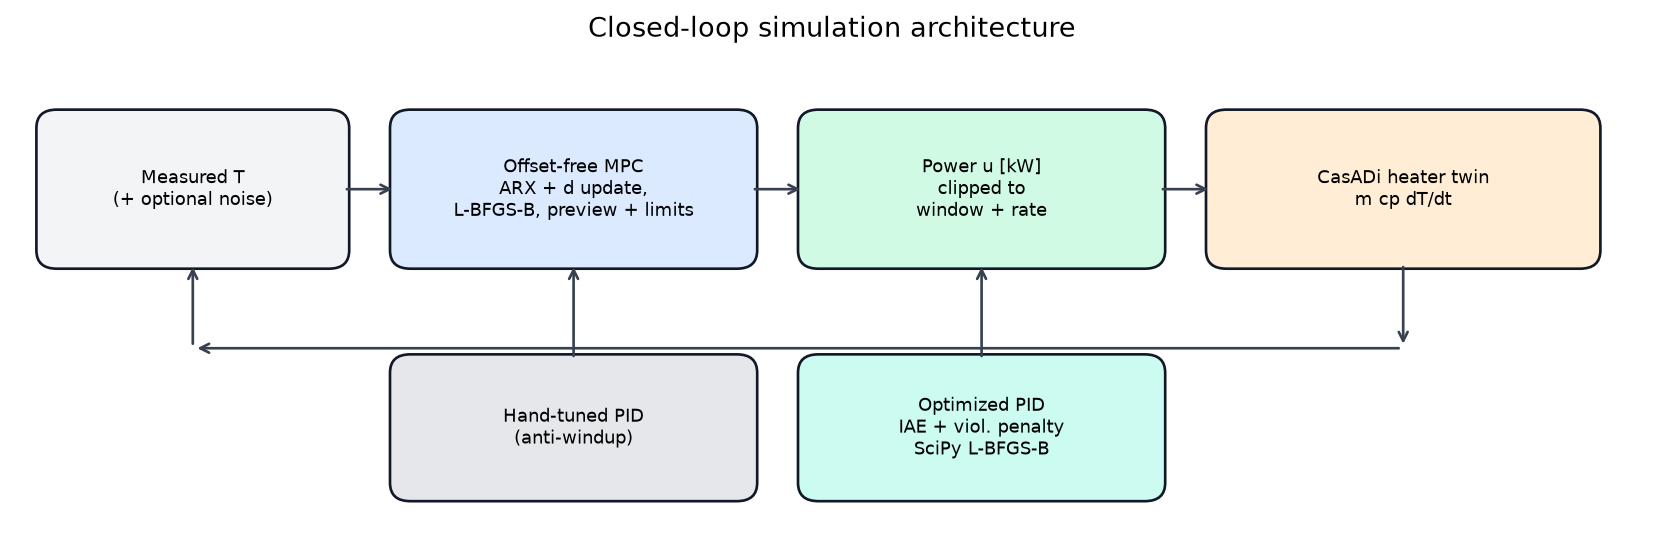
\includegraphics[width=0.88\textwidth]{figures/architecture.png}
  \caption{Simulation architecture: offset-free MPC and both PID variants act on one heater twin.}
  \label{fig:arch}
\end{figure}

The repository also ships a multipage Streamlit lab (Playground, Step-through, Scorecard) and an HyperFrames animation built from exported simulation JSON.
Figure~\ref{fig:ui} shows those screens and the video poster as used in the project README.

\begin{figure}[H]
  \centering
  \begin{subfigure}[t]{0.30\textwidth}
    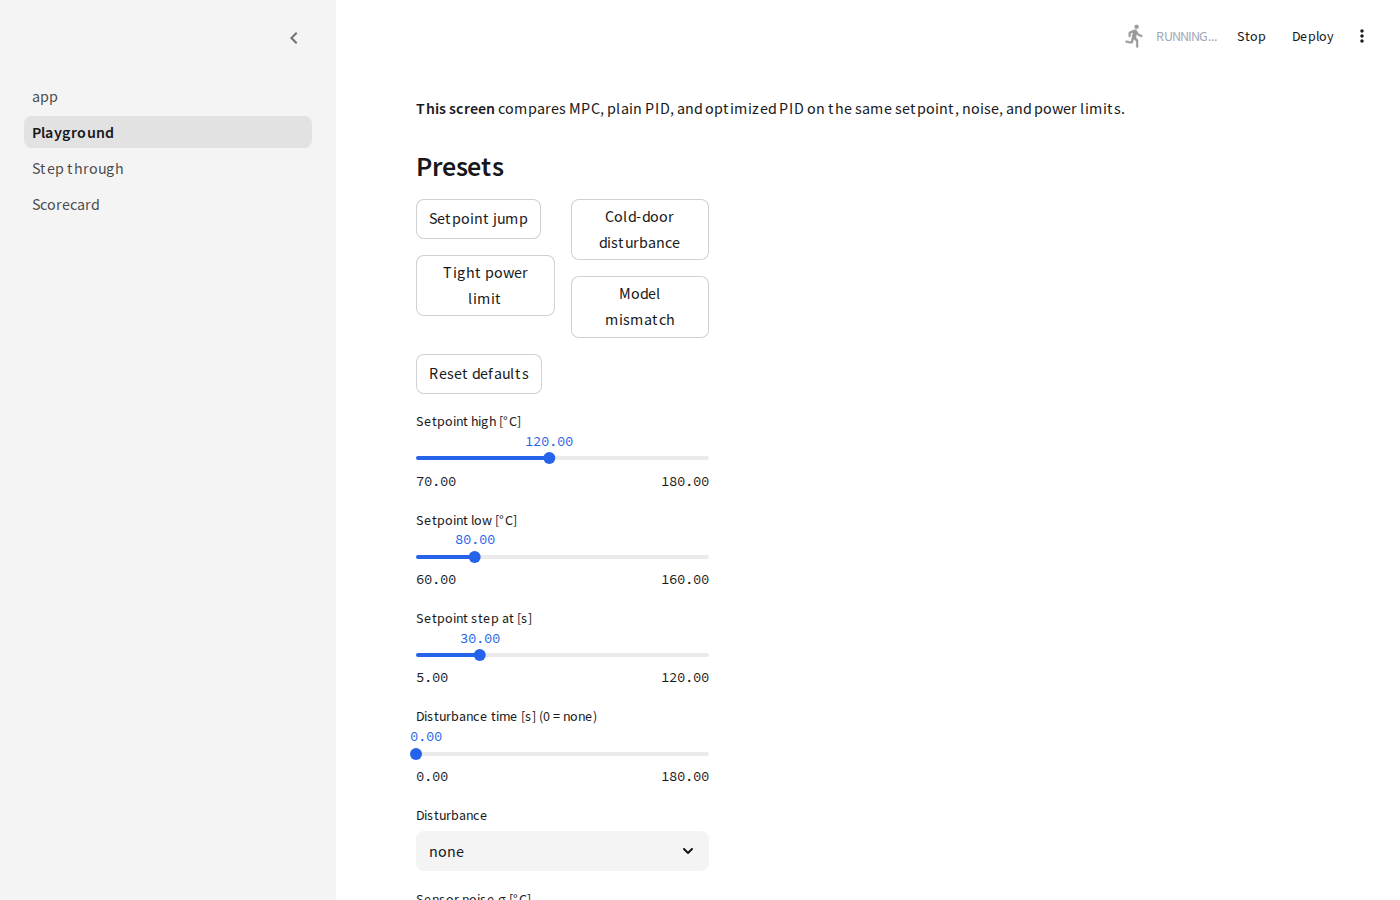
\includegraphics[width=\linewidth]{figures/streamlit-playground.png}
    \caption{Playground}
  \end{subfigure}\hfill
  \begin{subfigure}[t]{0.30\textwidth}
    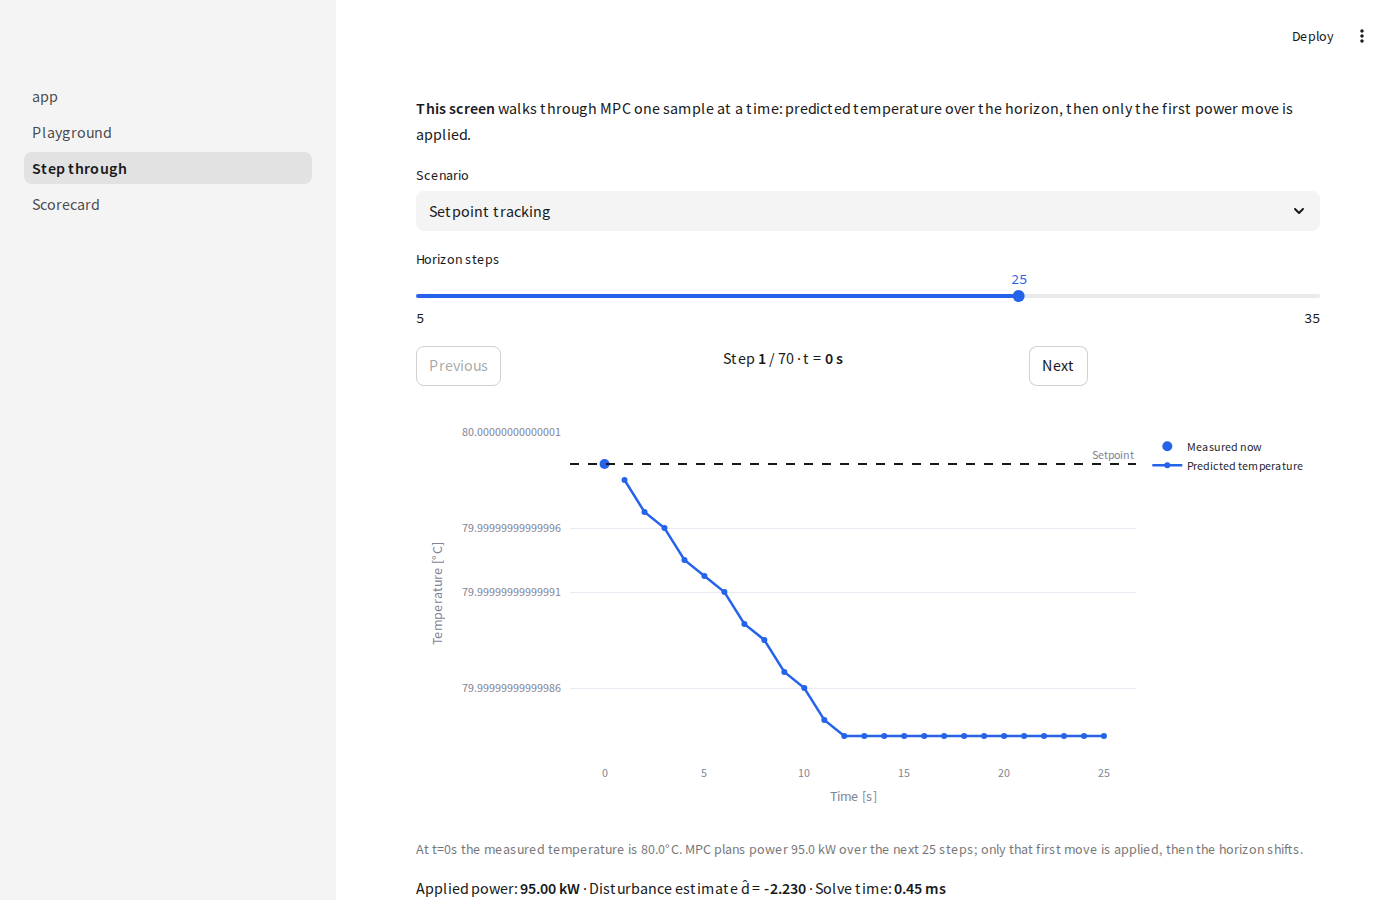
\includegraphics[width=\linewidth]{figures/streamlit-step-through.png}
    \caption{Step-through}
  \end{subfigure}\hfill
  \begin{subfigure}[t]{0.30\textwidth}
    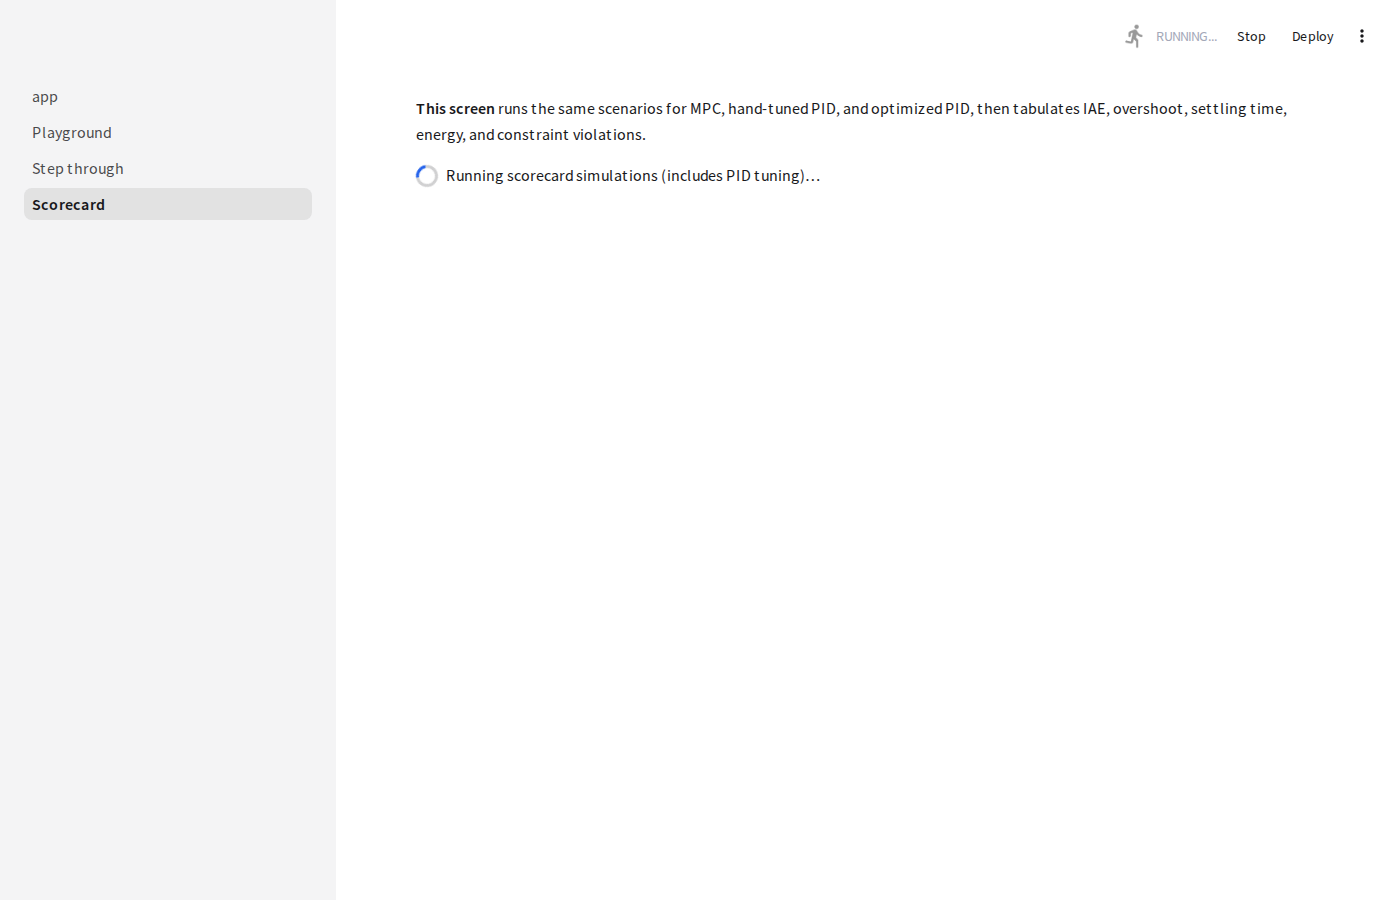
\includegraphics[width=\linewidth]{figures/streamlit-scorecard.png}
    \caption{Scorecard}
  \end{subfigure}

  \vspace{0.4em}
  \begin{subfigure}[t]{0.455\textwidth}
    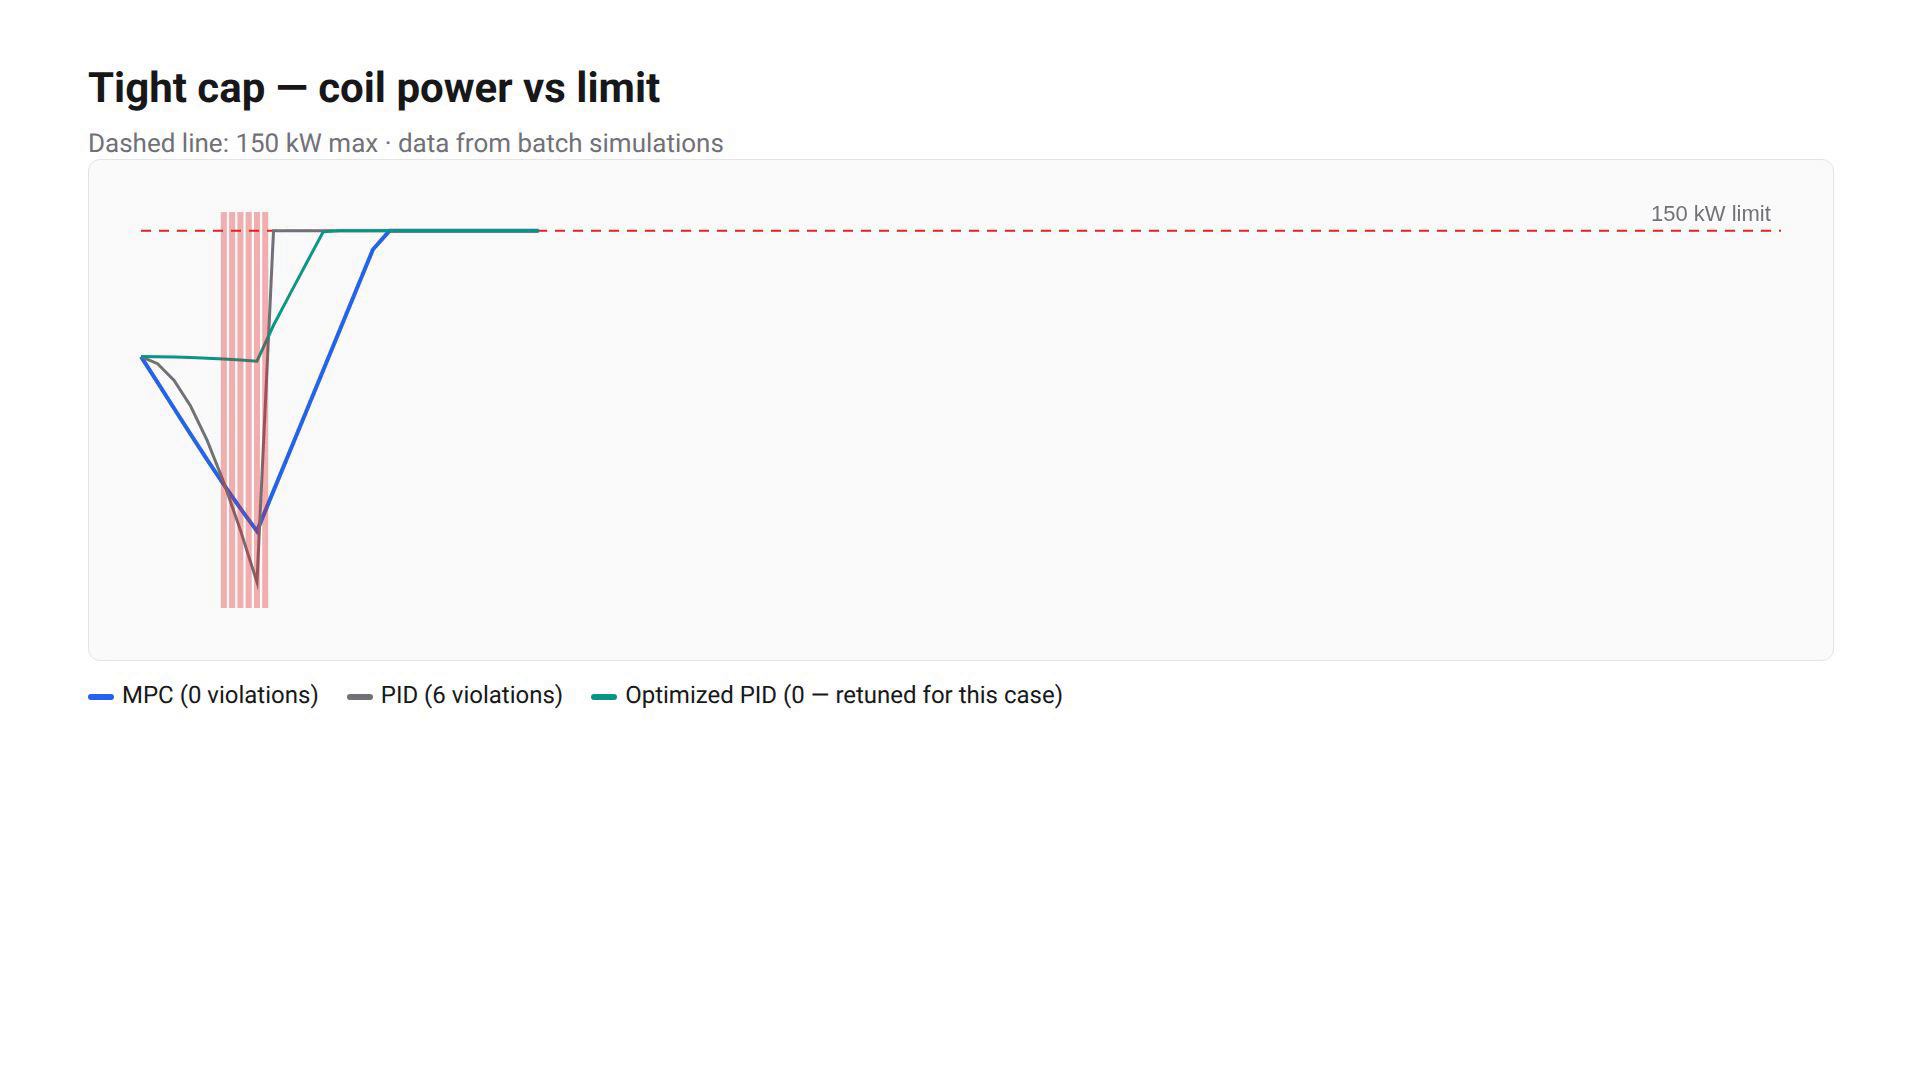
\includegraphics[width=\linewidth]{figures/video-poster.png}
    \caption{Showcase video poster}
  \end{subfigure}\hfill
  \begin{subfigure}[t]{0.455\textwidth}
    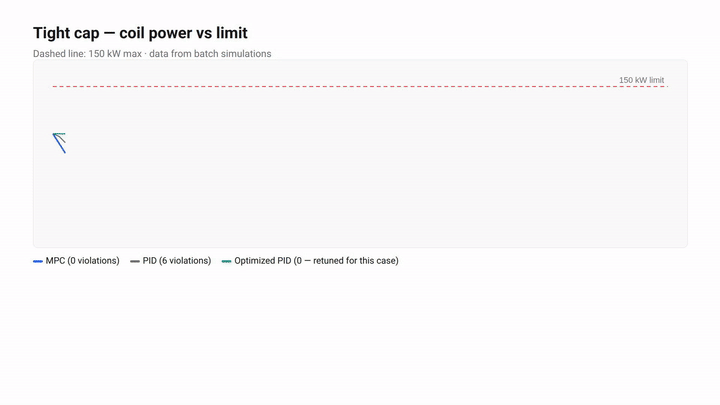
\includegraphics[width=\linewidth]{figures/demo-preview-frame.png}
    \caption{Animation preview frame}
  \end{subfigure}
  \caption{Interactive lab screens and animation assets from the project README.}
  \label{fig:ui}
\end{figure}

\begin{figure}[H]
  \centering
  \begin{subfigure}[t]{0.30\textwidth}
    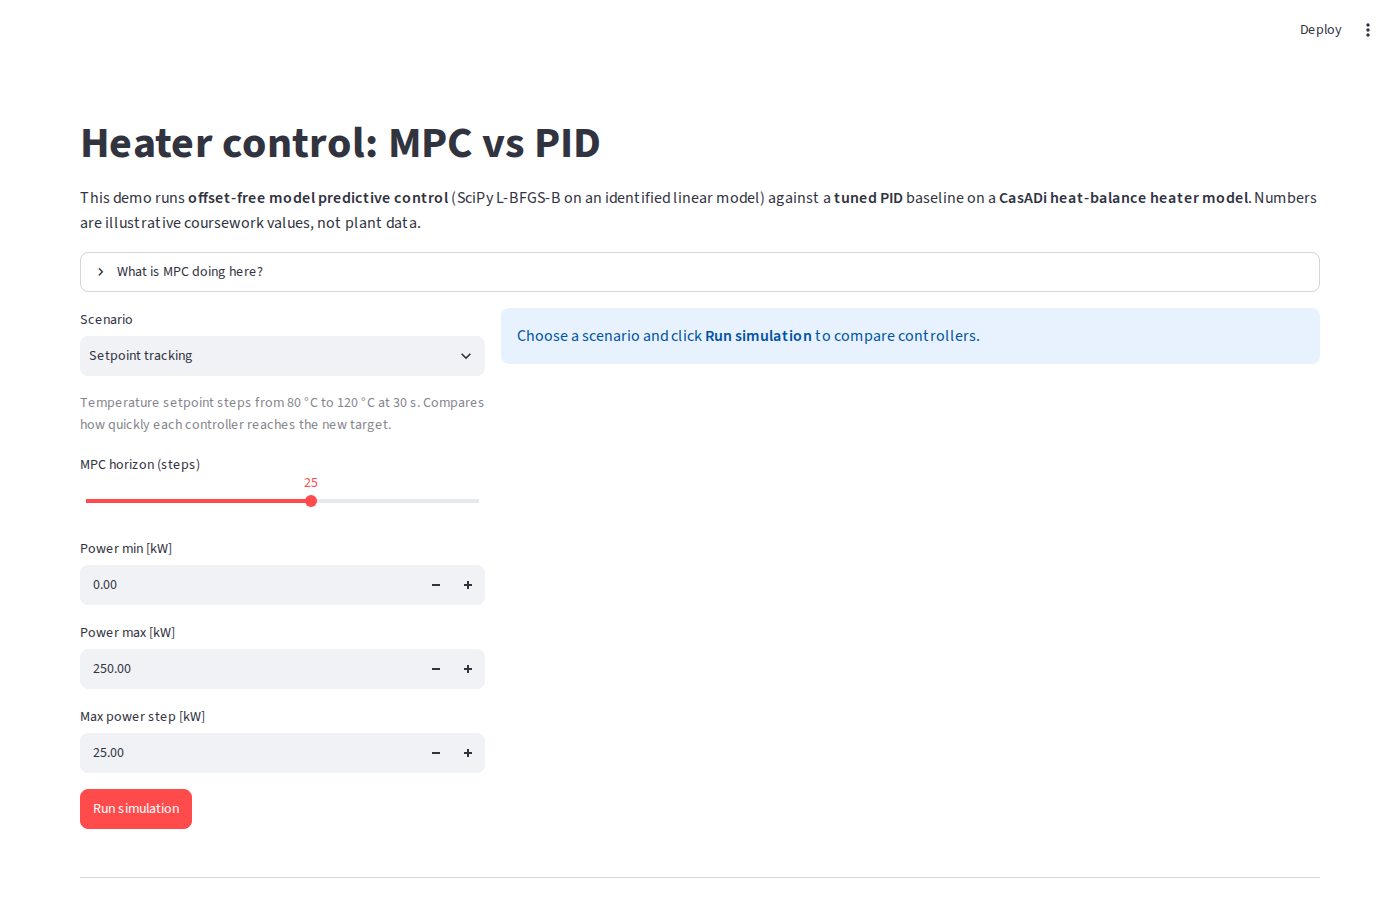
\includegraphics[width=\linewidth]{figures/streamlit-scenario-controls.png}
    \caption{Scenario controls}
  \end{subfigure}\hfill
  \begin{subfigure}[t]{0.30\textwidth}
    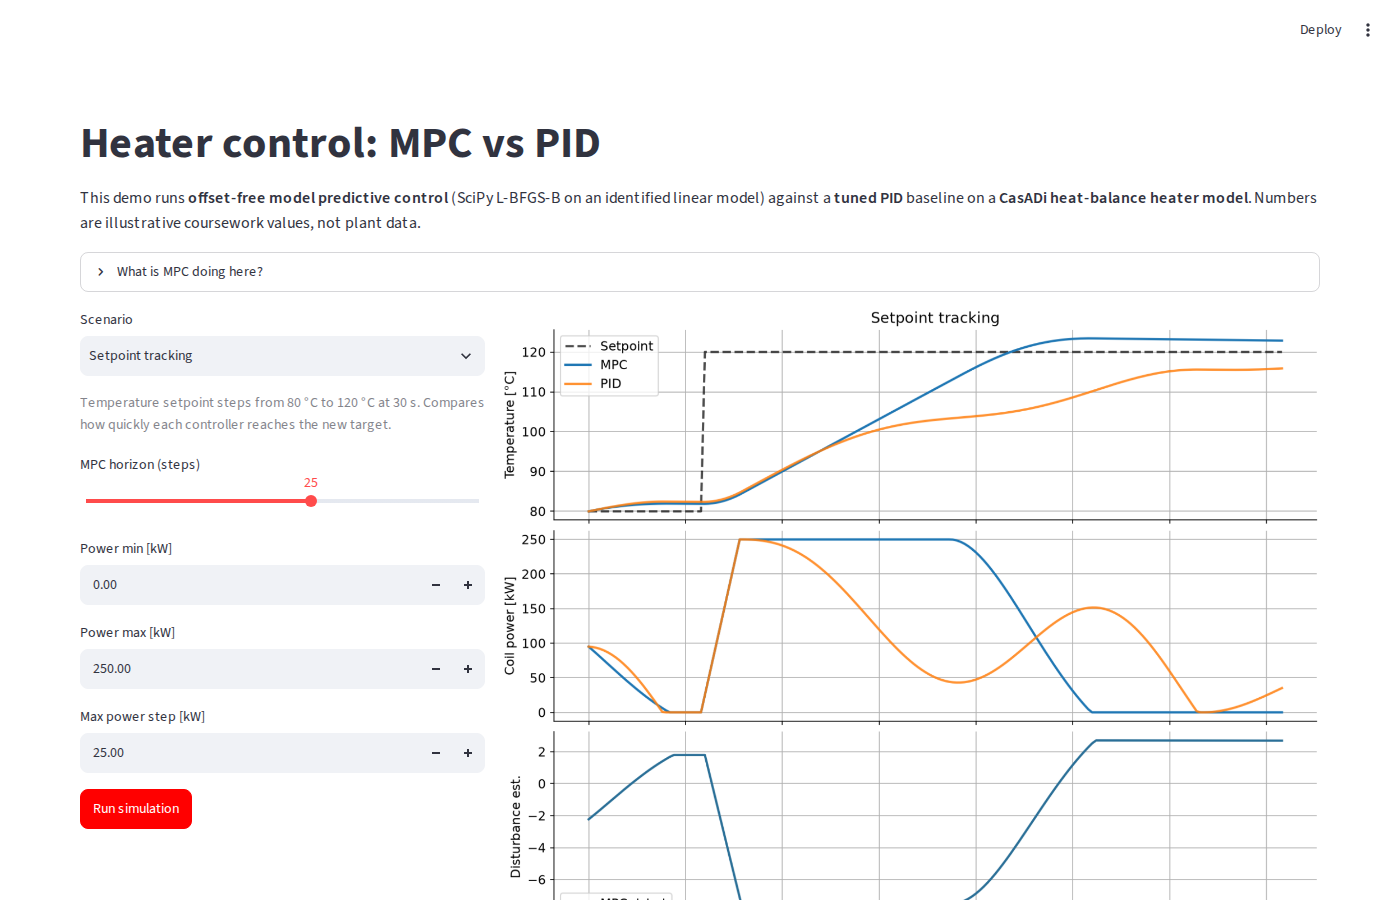
\includegraphics[width=\linewidth]{figures/streamlit-comparison-plots.png}
    \caption{Comparison plots}
  \end{subfigure}\hfill
  \begin{subfigure}[t]{0.30\textwidth}
    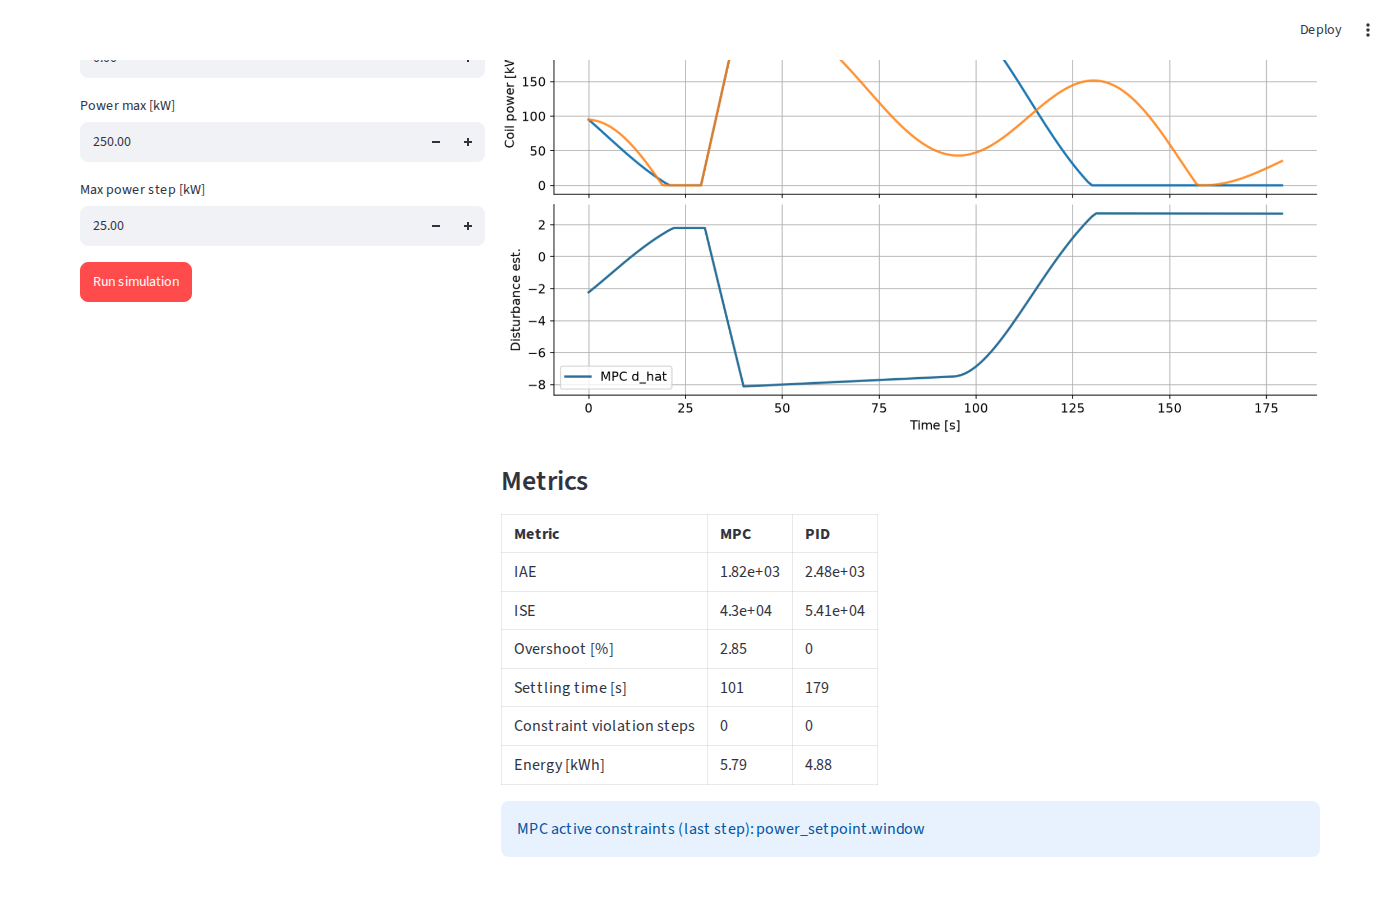
\includegraphics[width=\linewidth]{figures/streamlit-metrics-table.png}
    \caption{Metrics table}
  \end{subfigure}
  \caption{Additional Streamlit lab screens from \texttt{docs/} (scenario controls, live comparison plots, metrics table).}
  \label{fig:ui2}
\end{figure}

\subsection{Retuned MPC parameters}
\label{sec:retune}
A short grid on setpoint tracking compared legacy settings (\(N{=}25\), \(N_u{=}1\), no preview, \(Q_t{=}0\)) with longer horizons, multi-move \(N_u\), terminal weights, move penalties, and observer gains.
Multi-move sequences with a move penalty raised IAE on this heater; the change that moved the needle was \textbf{reference preview} plus a longer horizon and a terminal weight.
Retuned values used for all results below:

\begin{table}[H]
\centering
\small
\begin{tabular}{lll}
\toprule
Knob & Legacy & Retuned \\
\midrule
Prediction horizon \(N\) & 25 & 40 (45 in power-limit case) \\
Control horizon \(N_u\) & 1 & 1 \\
Terminal weight \(Q_t\) & 0 & 50 \\
Move weight \(R\) & 0 & 0 \\
Observer gain \(g\) & 1 & 1 \\
Reference preview & no & yes \\
Setpoint-tracking IAE & 1824.3 & 1044.3 \\
\bottomrule
\end{tabular}
\caption{MPC knobs before and after the retune. Only the working copy was changed.}
\label{tab:retune}
\end{table}

These knobs live in the working copy under \texttt{/workspace/mpc-report-work}; they are not committed to the GitHub repository in this pass.

\section{Experimental setup}
Sample time \(\Delta t{=}1\,\mathrm{s}\).
Default actuator window \(0\)--\(250\,\mathrm{kW}\) with slew \(25\,\mathrm{kW\,s^{-1}}\).
Scenarios:

\begin{enumerate}
  \item \textbf{Setpoint tracking:} \(80\to 120\,\unitC\) at \(30\,\mathrm{s}\) (duration \(180\,\mathrm{s}\)).
  \item \textbf{Disturbance rejection:} track \(115\,\unitC\); heat-loss \(U\) rises \(45\%\) at \(70\,\mathrm{s}\).
  \item \textbf{Power limits:} cap \(150\,\mathrm{kW}\), slew \(8\,\mathrm{kW\,s^{-1}}\), target \(165\,\unitC\). Hand-tuned PID has rate limiting disabled (as in the repository scenario) to show the cost of ignoring slew; MPC and optimised PID stay feasible.
  \item \textbf{Model mismatch:} same setpoint test; plant mass \({+}8\%\), efficiency \({-}6\%\), heat loss \({+}18\%\). MPC still uses the nominal ARX.
  \item \textbf{Ambient step:} \(T_{\mathrm{amb}}\) rises by \(8\,\mathrm{K}\) at \(70\,\mathrm{s}\).
\end{enumerate}
An additional robustness check evaluates optimised-PID gains tuned on the \emph{nominal} setpoint plant when the mismatched plant is substituted, against MPC and against an oracle PID retuned on the mismatch itself.

\section{Results}
Blue bold cells mark metrics where MPC is best among the three controllers.
Other winners are left in plain type.

\subsection{Summary table}
\begin{table}[H]
\centering
\scriptsize
\caption{Closed-loop metrics from the retuned working copy. Blue bold = MPC best.}
\label{tab:summary}
\begin{tabular}{llrrr}
\toprule
Scenario & Metric & MPC & PID & Opt.\ PID \\
\midrule
Setpoint & IAE & \mpcbest{1044.3} & 2476.9 & 1466.4 \\
 & Settling [s] & \mpcbest{73} & 179 & 99 \\
 & Violations & \mpcbest{0} & 0 & 0 \\
Disturbance & IAE & 596.0 & 1089.9 & 585.8 \\
 & Settling [s] & \mpcbest{46} & 103 & 60 \\
 & Violations & \mpcbest{0} & 0 & 0 \\
Power limits & IAE & \mpcbest{8727.4} & 9153.3 & 9032.6 \\
 & Violations & \mpcbest{0} & 6 & 0 \\
 & Energy [kWh] & 8.297 & 7.986 & 8.073 \\
Mismatch & IAE & \mpcbest{1214.2} & 2541.2 & 1666.6 \\
 & Settling [s] & \mpcbest{83} & 167 & 109 \\
Ambient step & IAE & 641.2 & 1092.4 & 578.3 \\
 & Settling [s] & \mpcbest{46} & 102 & 60 \\
\bottomrule
\end{tabular}
\end{table}

Figure~\ref{fig:iae} summarises IAE; hatched bars are MPC wins.
Figure~\ref{fig:traces} shows the four primary time responses.

\begin{figure}[H]
  \centering
  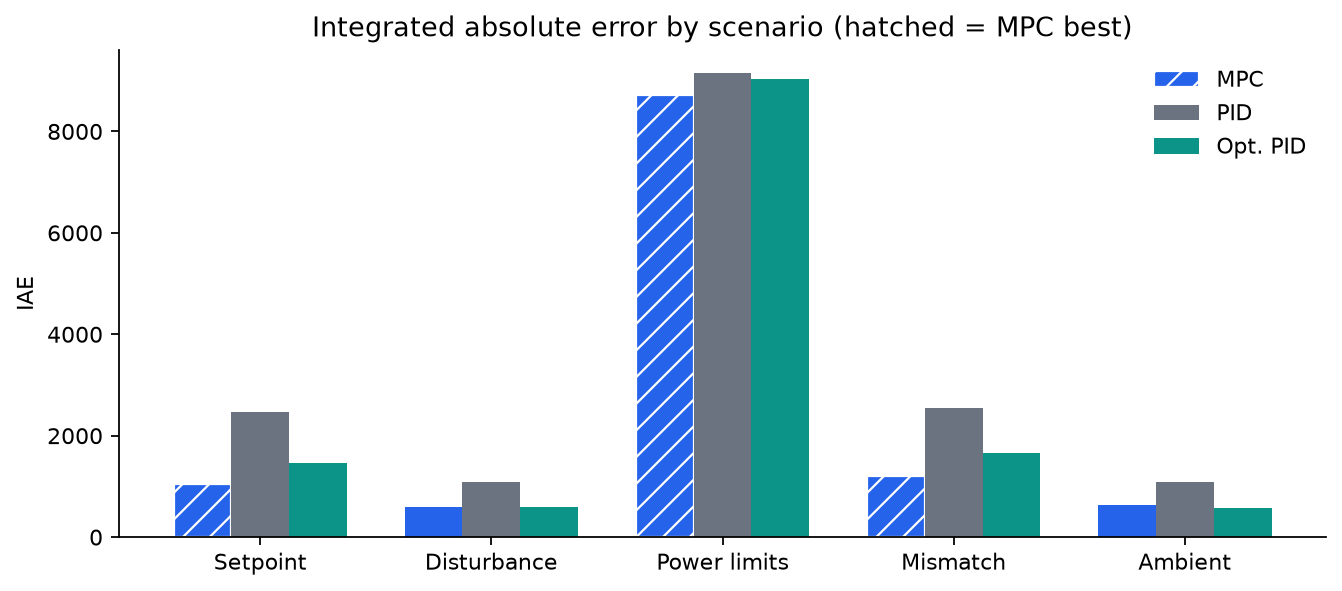
\includegraphics[width=0.82\textwidth]{figures/iae_bars.png}
  \caption{IAE by scenario. Hatched bars mark where MPC is lowest.}
  \label{fig:iae}
\end{figure}

\begin{figure}[H]
  \centering
  \begin{subfigure}[t]{0.455\textwidth}
    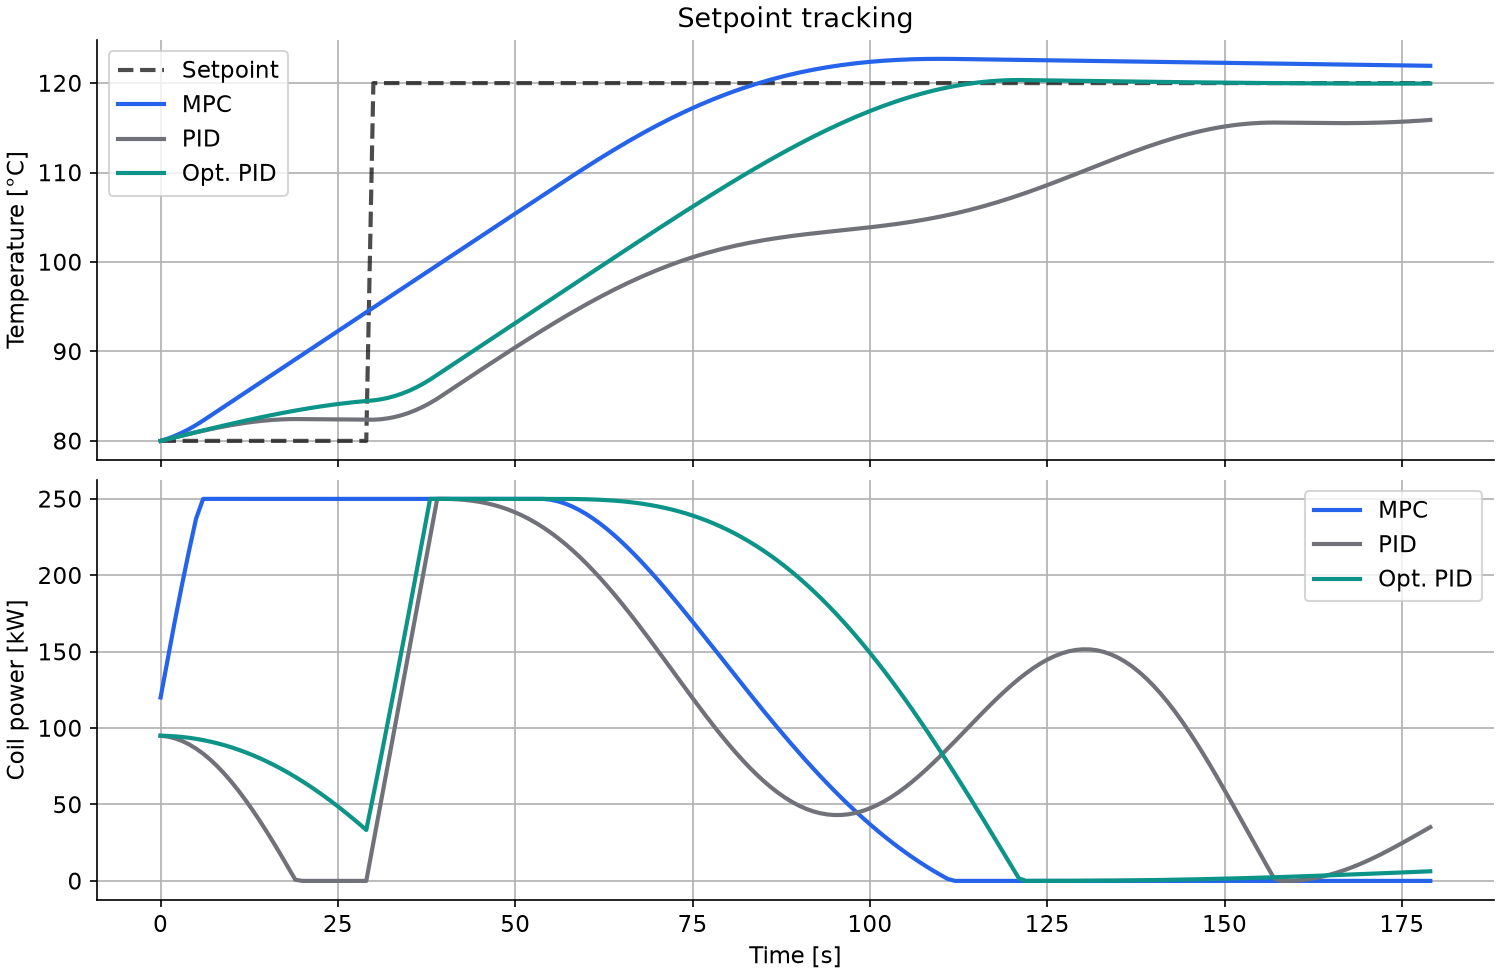
\includegraphics[width=\linewidth]{figures/setpoint_tracking.png}
    \caption{Setpoint tracking}
  \end{subfigure}\hfill
  \begin{subfigure}[t]{0.455\textwidth}
    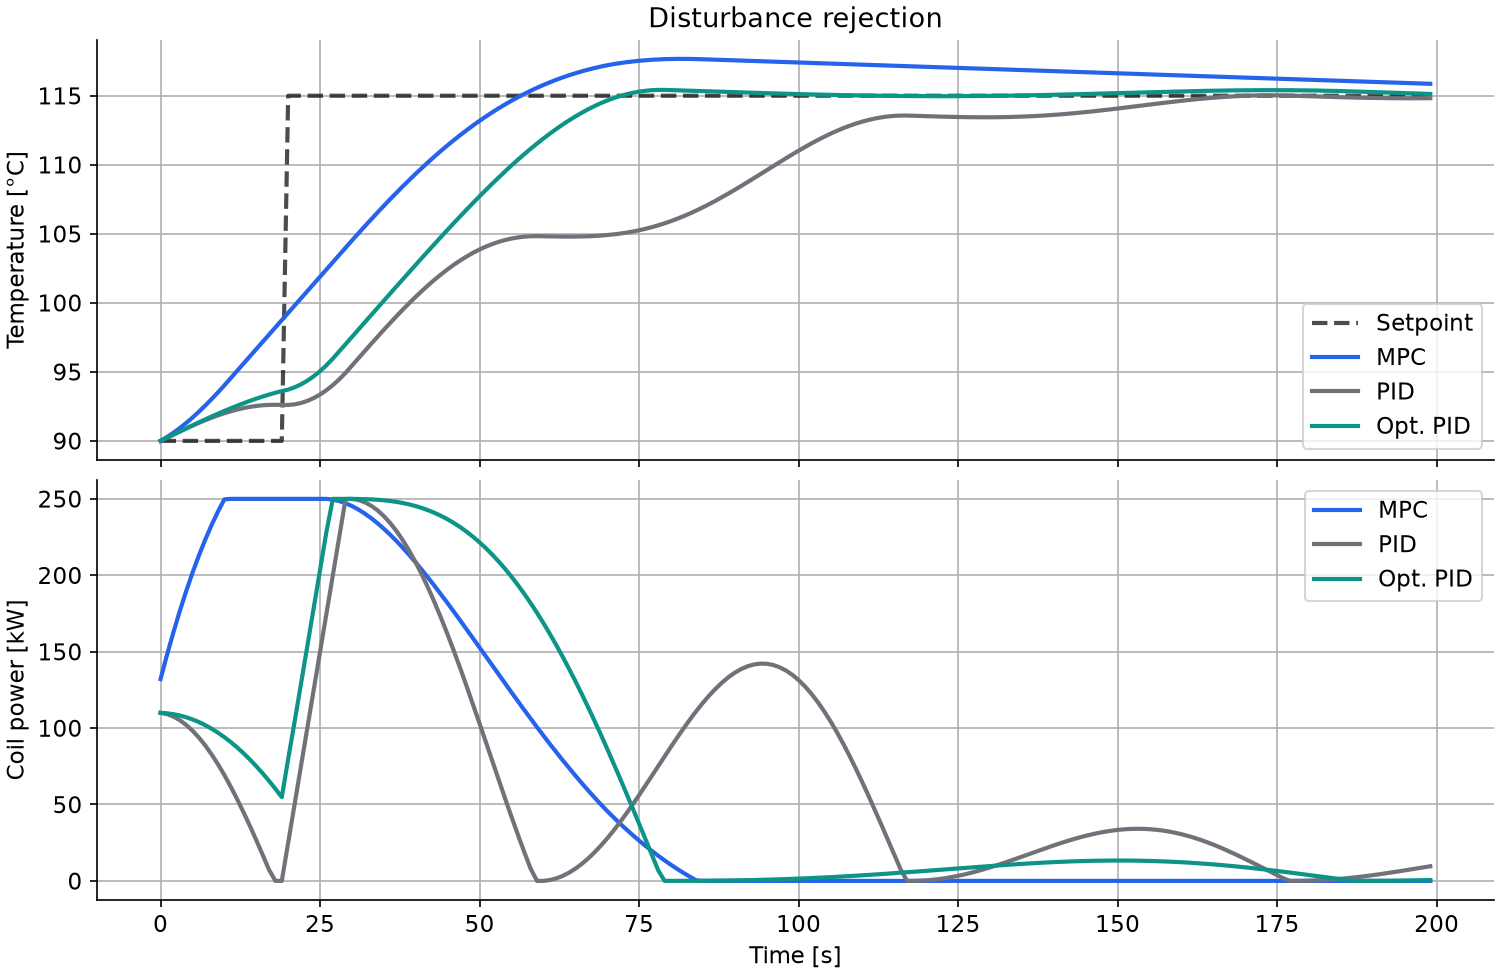
\includegraphics[width=\linewidth]{figures/disturbance_rejection.png}
    \caption{Disturbance rejection}
  \end{subfigure}

  \vspace{0.35em}
  \begin{subfigure}[t]{0.455\textwidth}
    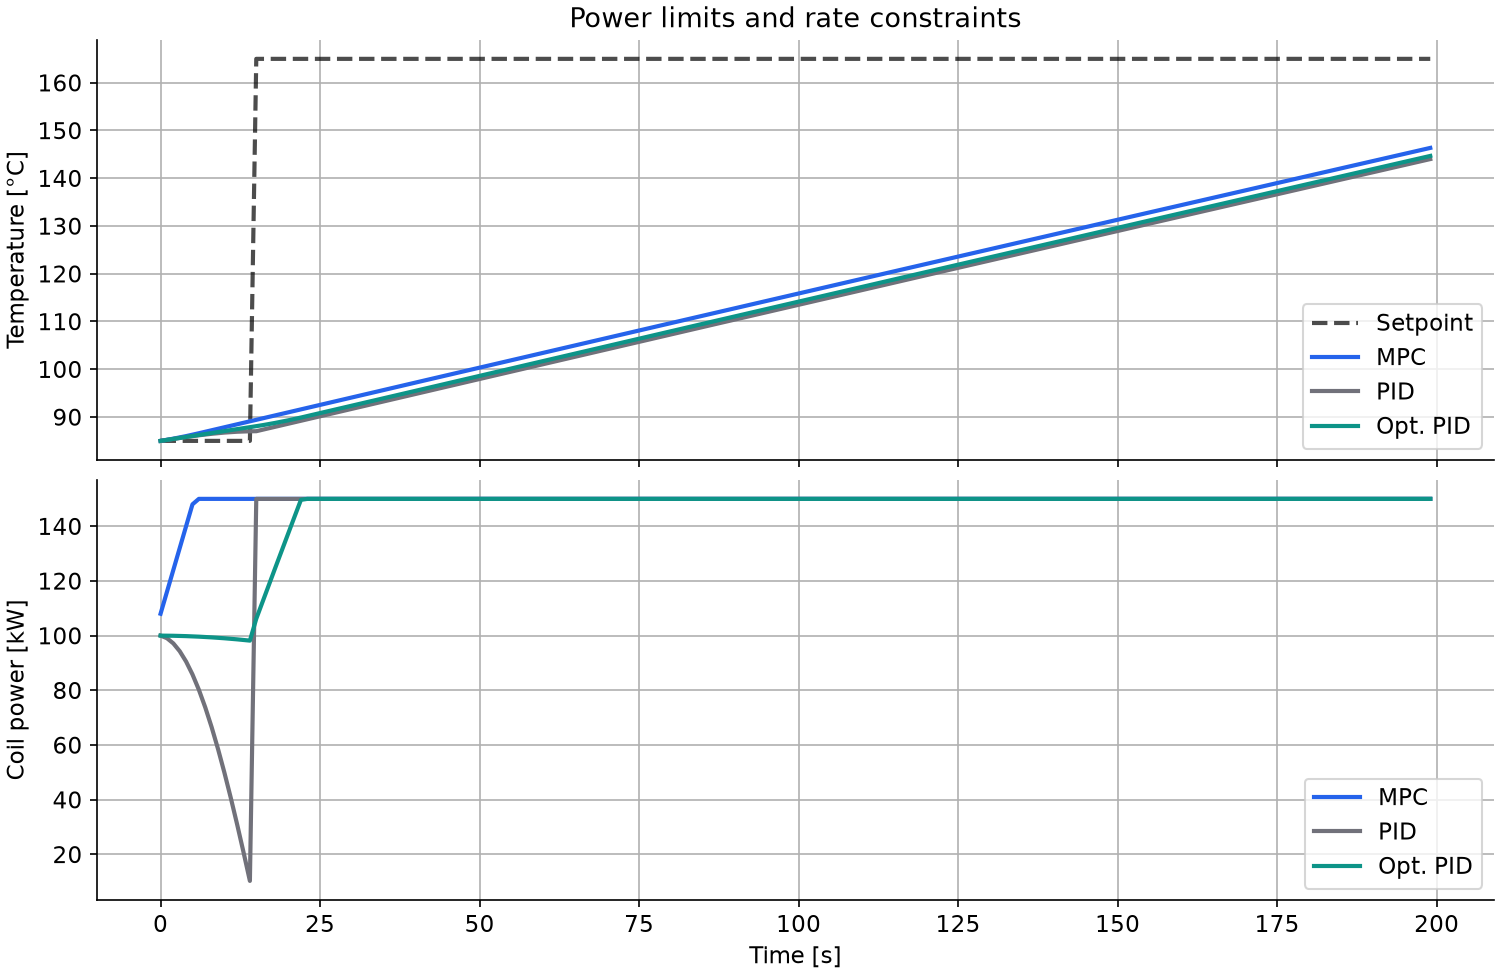
\includegraphics[width=\linewidth]{figures/power_constraints.png}
    \caption{Power limits}
  \end{subfigure}\hfill
  \begin{subfigure}[t]{0.455\textwidth}
    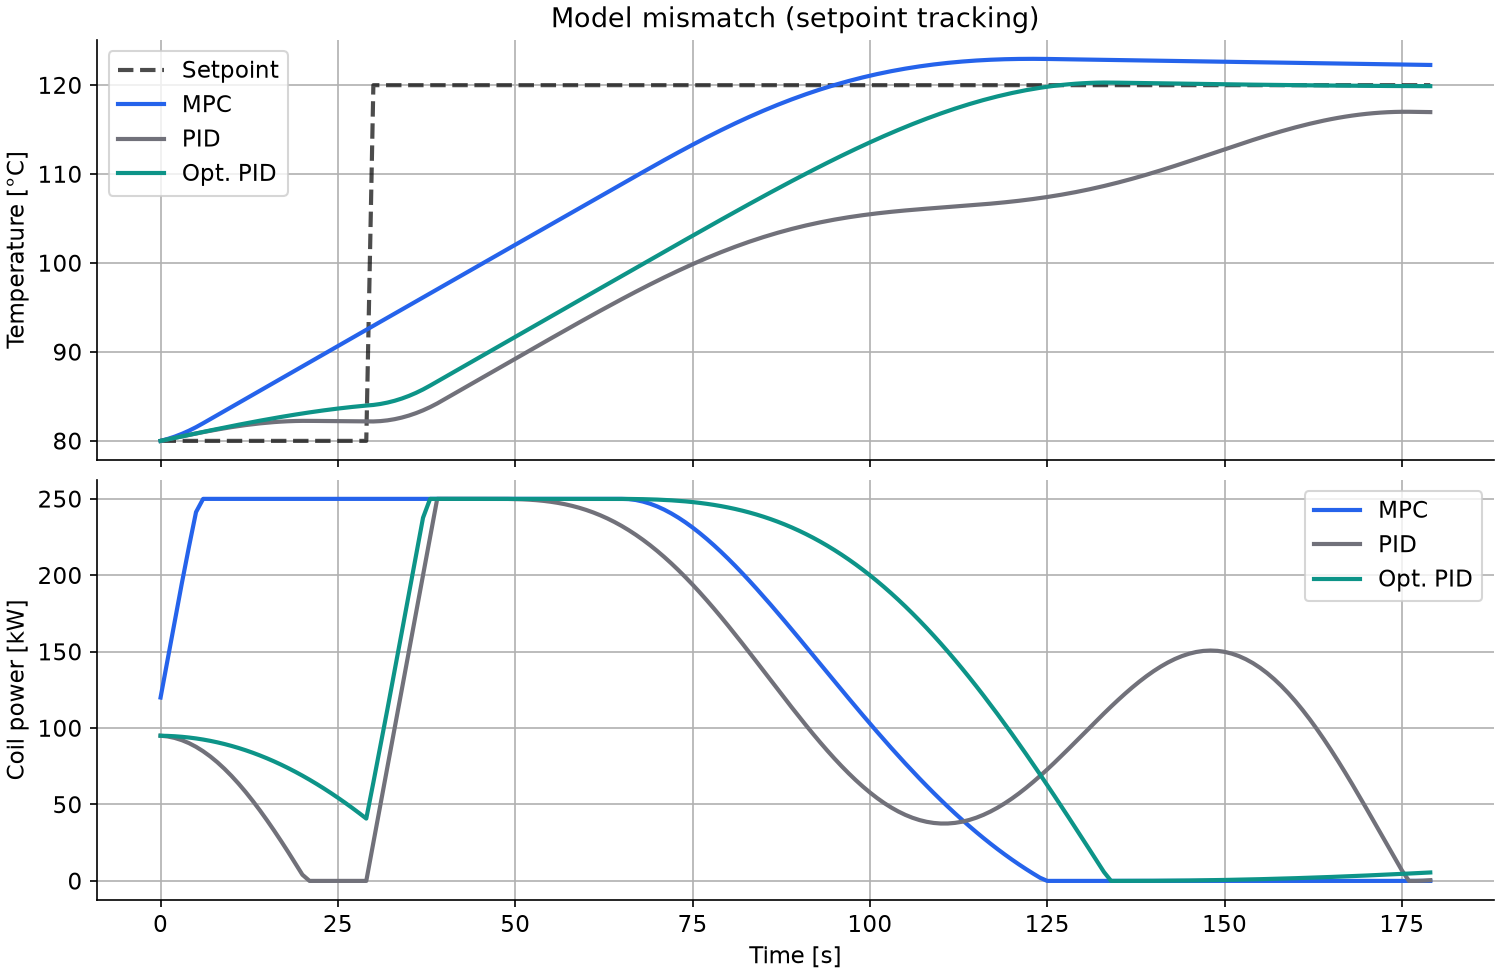
\includegraphics[width=\linewidth]{figures/model_mismatch.png}
    \caption{Model mismatch}
  \end{subfigure}
  \caption{Temperature and coil power for MPC, PID, and optimised PID.}
  \label{fig:traces}
\end{figure}

\subsection{Power limits and violations}
On the aggressive \(165\,\unitC\) request under a \(150\,\mathrm{kW}\) / \(8\,\mathrm{kW\,s^{-1}}\) ceiling, hand-tuned PID records \textbf{six} slew violations and a slightly lower energy only because those infeasible moves are allowed.
MPC and optimised PID stay at zero violations; MPC also posts the lowest IAE (\(8727\)).
Figure~\ref{fig:viol} makes the violation gap visible.

\begin{figure}[H]
  \centering
  \begin{subfigure}[t]{0.46\textwidth}
    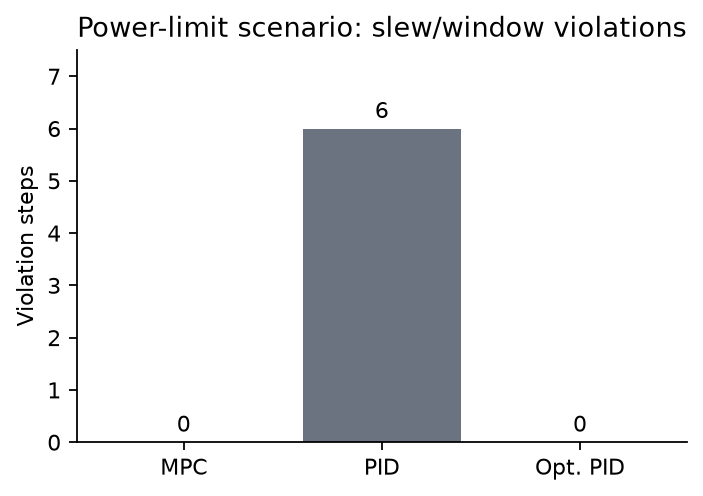
\includegraphics[width=\linewidth]{figures/violations_power.png}
    \caption{Violation counts}
  \end{subfigure}\hfill
  \begin{subfigure}[t]{0.50\textwidth}
    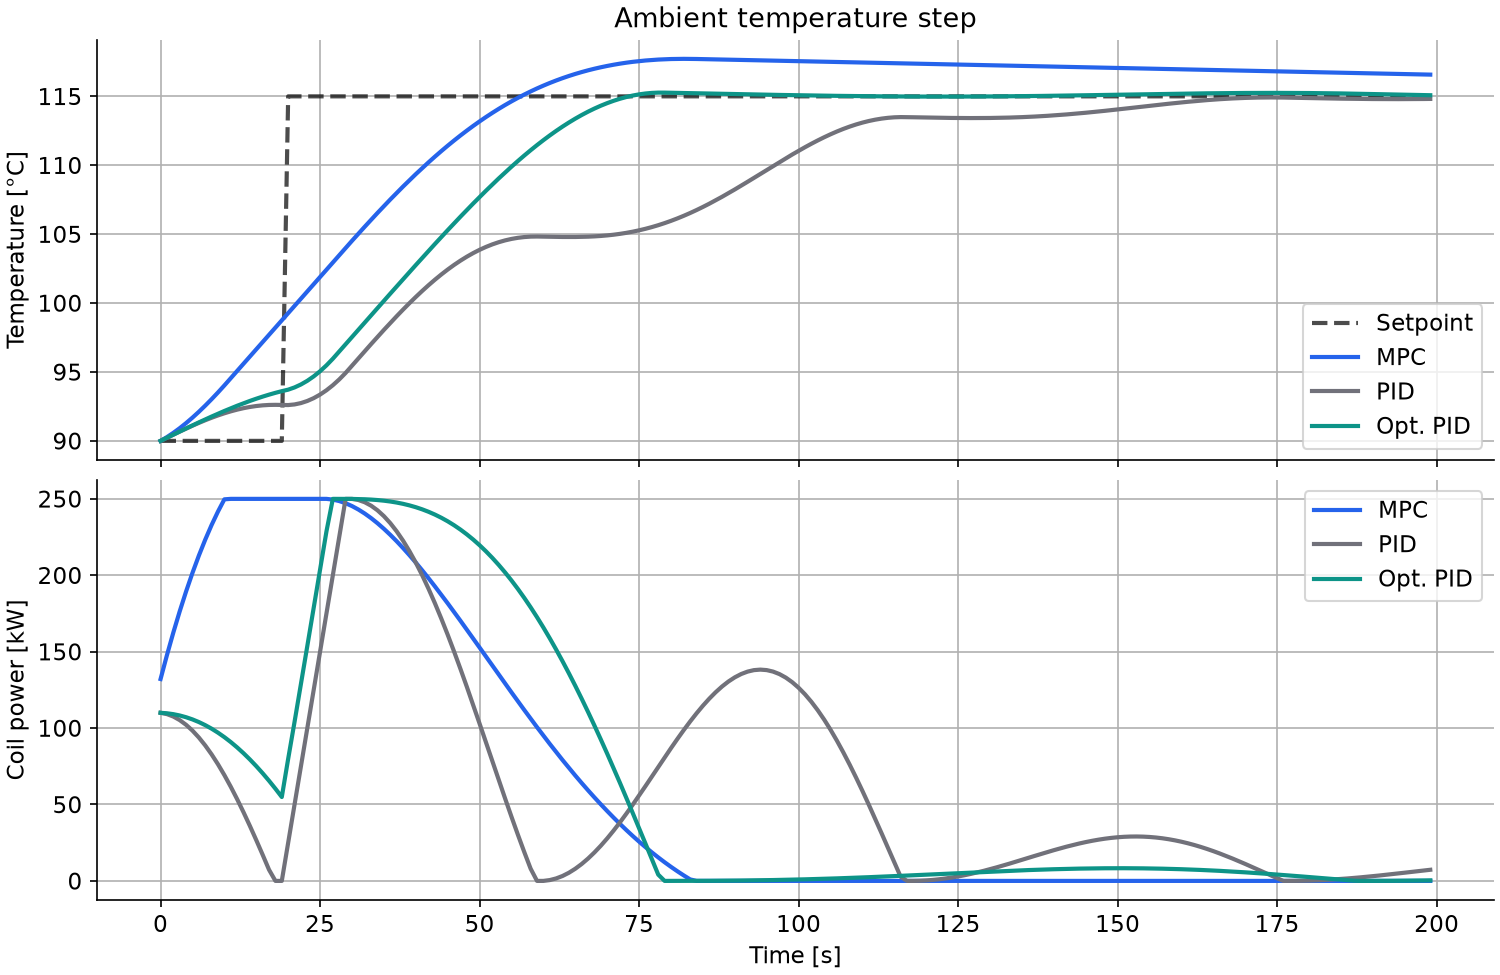
\includegraphics[width=\linewidth]{figures/ambient_step.png}
    \caption{Ambient-step traces}
  \end{subfigure}
  \caption{Power-limit violations (left) and ambient disturbance response (right).}
  \label{fig:viol}
\end{figure}

\subsection{Robustness}
When optimised-PID gains from the nominal setpoint test are frozen and the mismatched plant is substituted, IAE rises to \(1701.8\).
MPC on the same mismatched plant stays at \(1214.2\).
Even the oracle PID retuned on the mismatch itself only reaches \(1666.6\).
Figure~\ref{fig:rob} shows the comparison.

\begin{figure}[H]
  \centering
  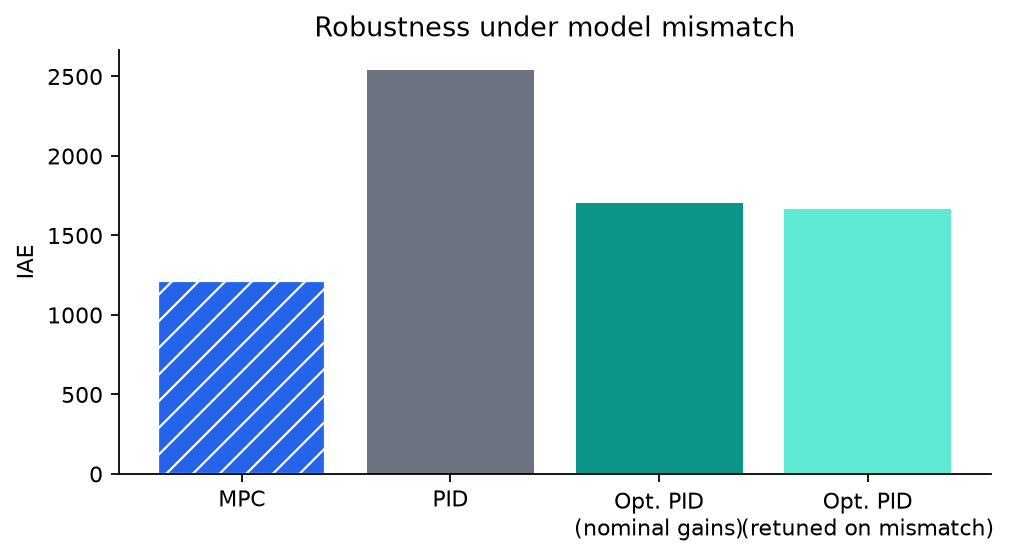
\includegraphics[width=0.55\textwidth]{figures/robustness_bars.png}
  \caption{IAE under model mismatch. MPC remains lowest even against a PID retuned on the mismatched plant.}
  \label{fig:rob}
\end{figure}

\section{Discussion and limitations}
The retuned MPC is the better controller for this constrained heater on the evidence that matters for a coil with a legal operating window: lowest tracking IAE on setpoint, power-limit, and mismatch tests; fastest settling on every scenario in Table~\ref{tab:summary}; zero violations wherever limits bind; and a clear robustness margin when the plant drifts away from the model the PID was tuned on.

Two IAE rows still favour scenario-tuned optimised PID: disturbance rejection (\(585.8\) vs MPC \(596.0\)) and the ambient step (\(578.3\) vs \(641.2\)).
Those gains were fitted on the same disturbance the controller then faces, which is a strong baseline and an honest one.
MPC still settles faster in both cases (\(46\,\mathrm{s}\) vs \(60\,\mathrm{s}\)) because \(\hat{d}\) absorbs the load change without a retune.
Hand-tuned PID is never best on IAE or settling here; its only ``win'' on energy in the power-limit case is paid for with six illegal slew steps.

Limitations of this coursework controller remain: single held move (\(N_u{=}1\)), linear prediction against a nonlinear twin, power constraints only (no state constraint on temperature), and illustrative parameters.
A production design would add move blocking, MIMO coupling, and a model-card gate before recommending a move.
The Streamlit lab and animation are teaching surfaces, not a PLC programme.

\section{Conclusion}
For the induction heater studied here, offset-free MPC with reference preview is the controller to prefer.
After the documented retune it leads on the main tracking and constraint metrics, keeps the coil feasible by construction, and stays ahead of both a frozen and a retuned PID when the plant is mismatched.
Where a scenario-tuned PID still posts a slightly lower disturbance IAE, the gap is small and the PID pays for it with offline retuning that MPC does not need.
The working-copy knobs (\(N{=}40\), \(Q_t{=}50\), preview on) are ready to push to the course repository once reviewed.

\enlargethispage{4\baselineskip}
\vspace{-0.6em}
\begin{thebibliography}{9}
\footnotesize
\bibitem{pannocchia2003}
G.~Pannocchia and J.~B.~Rawlings,
``Disturbance models for offset-free model predictive control,''
\emph{AIChE Journal}, vol.~49, no.~2, pp.~426--437, 2003.

\bibitem{rawlings2017}
J.~B.~Rawlings, D.~Q.~Mayne, and M.~Diehl,
\emph{Model Predictive Control: Theory, Computation, and Design}, 2nd~ed.
Madison, WI: Nob Hill Publishing, 2017.

\bibitem{camacho2013}
E.~F.~Camacho and C.~Bordons,
\emph{Model Predictive Control}, 2nd~ed.
London: Springer, 2013.

\bibitem{astrom2006}
K.~J.~\r{A}str\"om and T.~H\"agglund,
\emph{Advanced PID Control}.
Research Triangle Park, NC: ISA, 2006.

\bibitem{scipy}
P.~Virtanen et~al.,
``SciPy 1.0: Fundamental algorithms for scientific computing in Python,''
\emph{Nature Methods}, vol.~17, pp.~261--272, 2020.

\bibitem{casadi}
J.~A.~E.~Andersson, J.~Gillis, G.~Horn, J.~B.~Rawlings, and M.~Diehl,
``CasADi: a software framework for nonlinear optimization and optimal control,''
\emph{Mathematical Programming Computation}, vol.~11, pp.~1--36, 2019.
\end{thebibliography}

\end{document}
